\section{Experimental evaluation}

\subsection{Used datasets and methods}
All the datasets, hyperparameter values, etc.

\subsection{Evaluation of the adaptive approach}
Show the results of the adaptive prolongation on multiple datasets, compare it to ordinary Node2vec and HARP.

Possibly include statistical significance testing.

\begin{figure}
  \centering
  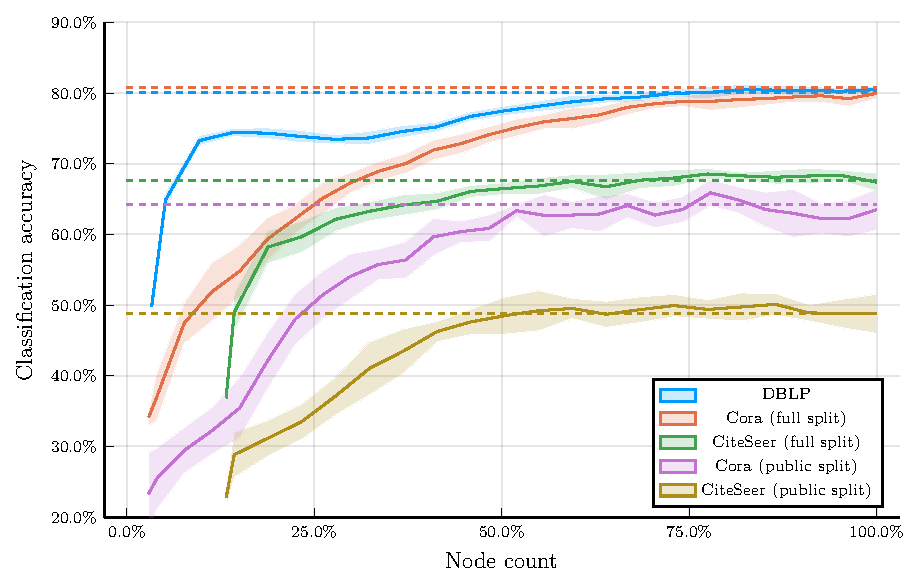
\includegraphics[width=\linewidth]{images/adaptive-coarsening/adaptive-coarsening.pdf}
  \caption{Adaptive coarsening results}
  \label{fig:adaptive-coarsening}
\end{figure}

\subsection{Relation to graph properties}

Compare the adaptive coarsening with local graph measures of graph homophilly

\subsection{Comparison of coarsening approaches}
